
\section{Architecture Integration}

\subsection{Model Support}

\begin{table}[H]
\centering
\small
\begin{tabular}{llllll}
\toprule
\textbf{Model} & \textbf{Attention class} & \textbf{Nested?} & \textbf{RoPE?} & \textbf{GQA?} & \textbf{Verified} \\
\midrule
DistilBERT & \texttt{MultiHeadSelfAttention} & No & No & No &  \\
RoBERTa & \texttt{BertSelfAttention} (nested) & Yes & No & No &  \\
GPT-2 & \texttt{GPT2Attention} (Conv1D) & No & No & No &  \\
Qwen3.5 & \texttt{Qwen3Attention} & No & Yes & Yes & 0.85 \\
\bottomrule
\end{tabular}
\end{table}

\subsection{Weight Resolution}

EAT resolves \texttt{hidden\_size} and \texttt{num\_heads} in this order:

\begin{enumerate}
\item \texttt{config.hidden\_size} / \texttt{config.num\_attention\_heads}
\item From \texttt{source\_attn} projections (\texttt{q\_lin.in\_features}, etc.)
\item From \texttt{kwargs} (\texttt{hidden\_size}, \texttt{num\_heads})
\item Default \texttt{768} / \texttt{12}

\end{enumerate}
This ensures EAT works even when \texttt{config} is incomplete.

\subsection{Layer Targeting}

The injection hook searches for attention modules in this order:

\begin{enumerate}
\item \texttt{layer.attention} (RoBERTa/BERT)
\item \texttt{layer.self\_attn} (Qwen/LLaMA)
\item \texttt{layer.attn} (GPT-2)
\item \texttt{layer.self} (DistilBERT variants)

\end{enumerate}
For nested encoders, \texttt{layer.attention.self} is targeted.

\subsection{Copy Weights -- Case by Case}

\subsubsection{DistilBERT}

\begin{lstlisting}
# Flat attention -- all four projections available
extracted["q"] = (src.q\_lin.weight.data, src.q\_lin.bias.data)
extracted["k"] = (src.k\_lin.weight.data, src.k\_lin.bias.data)
extracted["v"] = (src.v\_lin.weight.data, src.v\_lin.bias.data)
extracted["o"] = (src.out\_lin.weight.data, src.out\_lin.bias.data)
\end{lstlisting}

\subsubsection{RoBERTa}

\begin{lstlisting}
# Nested -- extract from src.self, skip out\_proj
s = src.self
extracted["q"] = (s.query.weight.data, s.query.bias.data)
extracted["k"] = (s.key.weight.data, s.key.bias.data)
extracted["v"] = (s.value.weight.data, s.value.bias.data)
extracted["o"] = (src.output.dense.weight.data, src.output.dense.bias.data)
\end{lstlisting}

The \texttt{is\_nested\_encoder = True} flag means EAT returns the raw context 
without applying \texttt{out\_lin}. The outer \texttt{attention.output.dense} applies it.

\subsubsection{GPT-2}

\begin{lstlisting}
# Fused Conv1D -- transpose and split
w = src.c\_attn.weight.data.t()  # (3d, d)
q\_w, k\_w, v\_w = w.chunk(3, dim=0)
extracted["q"] = (q\_w, src.c\_attn.bias.data[:d])
extracted["k"] = (k\_w, src.c\_attn.bias.data[d:2*d])
extracted["v"] = (v\_w, src.c\_attn.bias.data[2*d:])
extracted["o"] = (src.c\_proj.weight.data.t(), src.c\_proj.bias.data)
\end{lstlisting}

\subsubsection{Qwen (GQA + RoPE)}

\begin{lstlisting}
# Direct copy from named projections
extracted["q"] = (src.q\_proj.weight.data, src.q\_proj.bias.data)
extracted["k"] = (src.k\_proj.weight.data, src.k\_proj.bias.data)
extracted["v"] = (src.v\_proj.weight.data, src.v\_proj.bias.data)
extracted["o"] = (src.o\_proj.weight.data, src.o\_proj.bias.data)
# RoPE preserved via rotary\_emb copy
\end{lstlisting}

\subsection{The `is\_nested\_encoder` Flag}

This flag determines whether the module applies its own \texttt{out\_lin} projection:

\begin{itemize}
\item \textbf{True} (RoBERTa): output projection is applied externally; EAT returns
  raw context.
\item \textbf{False} (DistilBERT, GPT-2, Qwen): EAT applies \texttt{out\_lin} internally.

\end{itemize}
\textbf{Common bug.} If \texttt{is\_nested\_encoder} is set incorrectly, the projection 
is applied twice (resulting in a scale collapse) or zero times (resulting 
in missing output).

The detection logic:

\begin{lstlisting}
if (hasattr(src, "self") and hasattr(src.self, "query")
    and hasattr(src, "output") and hasattr(src.output, "dense")):
    is\_nested = True
elif (cls\_name.endswith("SelfAttention") and "distil" not in cls\_name.lower()
      and not has\_out\_lin):
    is\_nested = True
\end{lstlisting}

\subsection{Injection}

\begin{lstlisting}
def inject\_eat(layer, model\_config=None, old\_attn=None, **kwargs):
    src = old\_attn or find\_attention(layer)
    new\_attn = EATBlock(config=model\_config, pretrained\_attn=src, **kwargs)
    replace\_attention(layer, new\_attn)
    return new\_attn
\end{lstlisting}

The replacement targets the same attribute path as the source:

\begin{lstlisting}
for attr in ("attention", "self\_attn", "attn", "self"):
    if hasattr(layer, attr):
        setattr(layer, attr, new\_attn)
        break
\end{lstlisting}

\subsection{Handling LoRA-Wrapped Source Modules}

If the source module is already wrapped with LoRA:

\begin{enumerate}
\item \textbf{Merge LoRA} into the base layer (\texttt{c\_attn\_mod.merge()}).
\item \textbf{Extract} merged weights.
\item \textbf{Re-initialize} LoRA in EAT with the same rank.

\end{enumerate}
This ensures the weights transferred are the effective weights, not the 
base weights.

\subsection{Failure Modes and Silent Fallback}

EAT's \texttt{copy\_weights} is defensive:

\begin{table}[H]
\centering
\small
\begin{tabular}{ll}
\toprule
\textbf{Failure} & \textbf{Action} \\
\midrule
LoRA merge fails & Log debug, continue with unmerged weights \\
Missing projection & Log warning, keep random init for that projection \\
Small Frobenius norm & Log warning, continue \\
UniversalAdapter fails & Log debug, continue \\
\bottomrule
\end{tabular}
\end{table}

\textbf{The critical consequence:} If weight transfer fails silently, EAT 
initializes with random weights, and the model's forward pass produces 
garbage. Recovery fine-tuning cannot compensate because gradient signals 
are dominated by noise.

\textbf{Mitigation.} We recommend:

\begin{enumerate}
\item \textbf{Add a hard assertion} (optional flag \texttt{strict\_weight\_transfer=True})
  that raises if any projection is missing.
\item \textbf{Post-injection sanity check:} Compare logits before and after
  injection on a fixed input. If the difference is large, abort.
\item \textbf{Log at WARN level} on any missing projection (currently does).

\end{enumerate}
\subsection{The `EATBlock` Module}

\begin{lstlisting}
class EATBlock(BaseAttention):
    def \_\_init\_\_(self, config, rank=64, ..., prune\_layer=None):
        super().\_\_init\_\_(config, rank)
        self.q\_lin = LoRALinear(d, H*d\_h, lora\_rank=16)
        self.k\_lin = LoRALinear(d, H\_kv*d\_h, lora\_rank=16)
        self.v\_lin = LoRALinear(d, H\_kv*d\_h, lora\_rank=16)
        self.out\_lin = LoRALinear(H*d\_h, d, lora\_rank=16)
        self.prune\_layer = prune\_layer
        if pretrained\_attn is not None:
            self.copy\_weights(pretrained\_attn)
    
    def forward(self, X, attention\_mask=None, ...):
        Q = self.q\_lin(X).view(...)
        K = self.k\_lin(X).view(...)
        V = self.v\_lin(X).view(...)
        # attention, output projection, optional pruning
        return Y
\end{lstlisting}

\subsection{Registry}

\begin{lstlisting}
@ATTENTION\_REGISTRY.register("eat")
@ATTENTION\_REGISTRY.register("eat\_attention")
class EATBlock(BaseAttention):
    ...
\end{lstlisting}

\subsection{Causality Verification}

For decoder models, EAT maintains causality because:

\begin{enumerate}
\item \textbf{Attention masking:} Causal mask is applied in \texttt{scores}.
\item \textbf{No future leakage in projections:} Q/K/V projections are
  position-wise.
\item \textbf{Pruning causality:} Progressive pruning, if used, must respect
  causal ordering (see \texttt{ProgressiveTokenPruning} documentation).

\end{enumerate}
\textbf{Verification.}

\begin{lstlisting}
X = torch.randn(1, L, d, requires\_grad=True)
Y = model(X)
loss = Y[0, i].sum()
loss.backward()
assert X.grad[0, i+1:].abs().max() \textless{} 1e-6
\end{lstlisting}

32
\begin{lstlisting}

---
\end{lstlisting}

\begin{figure}[H]
\centering
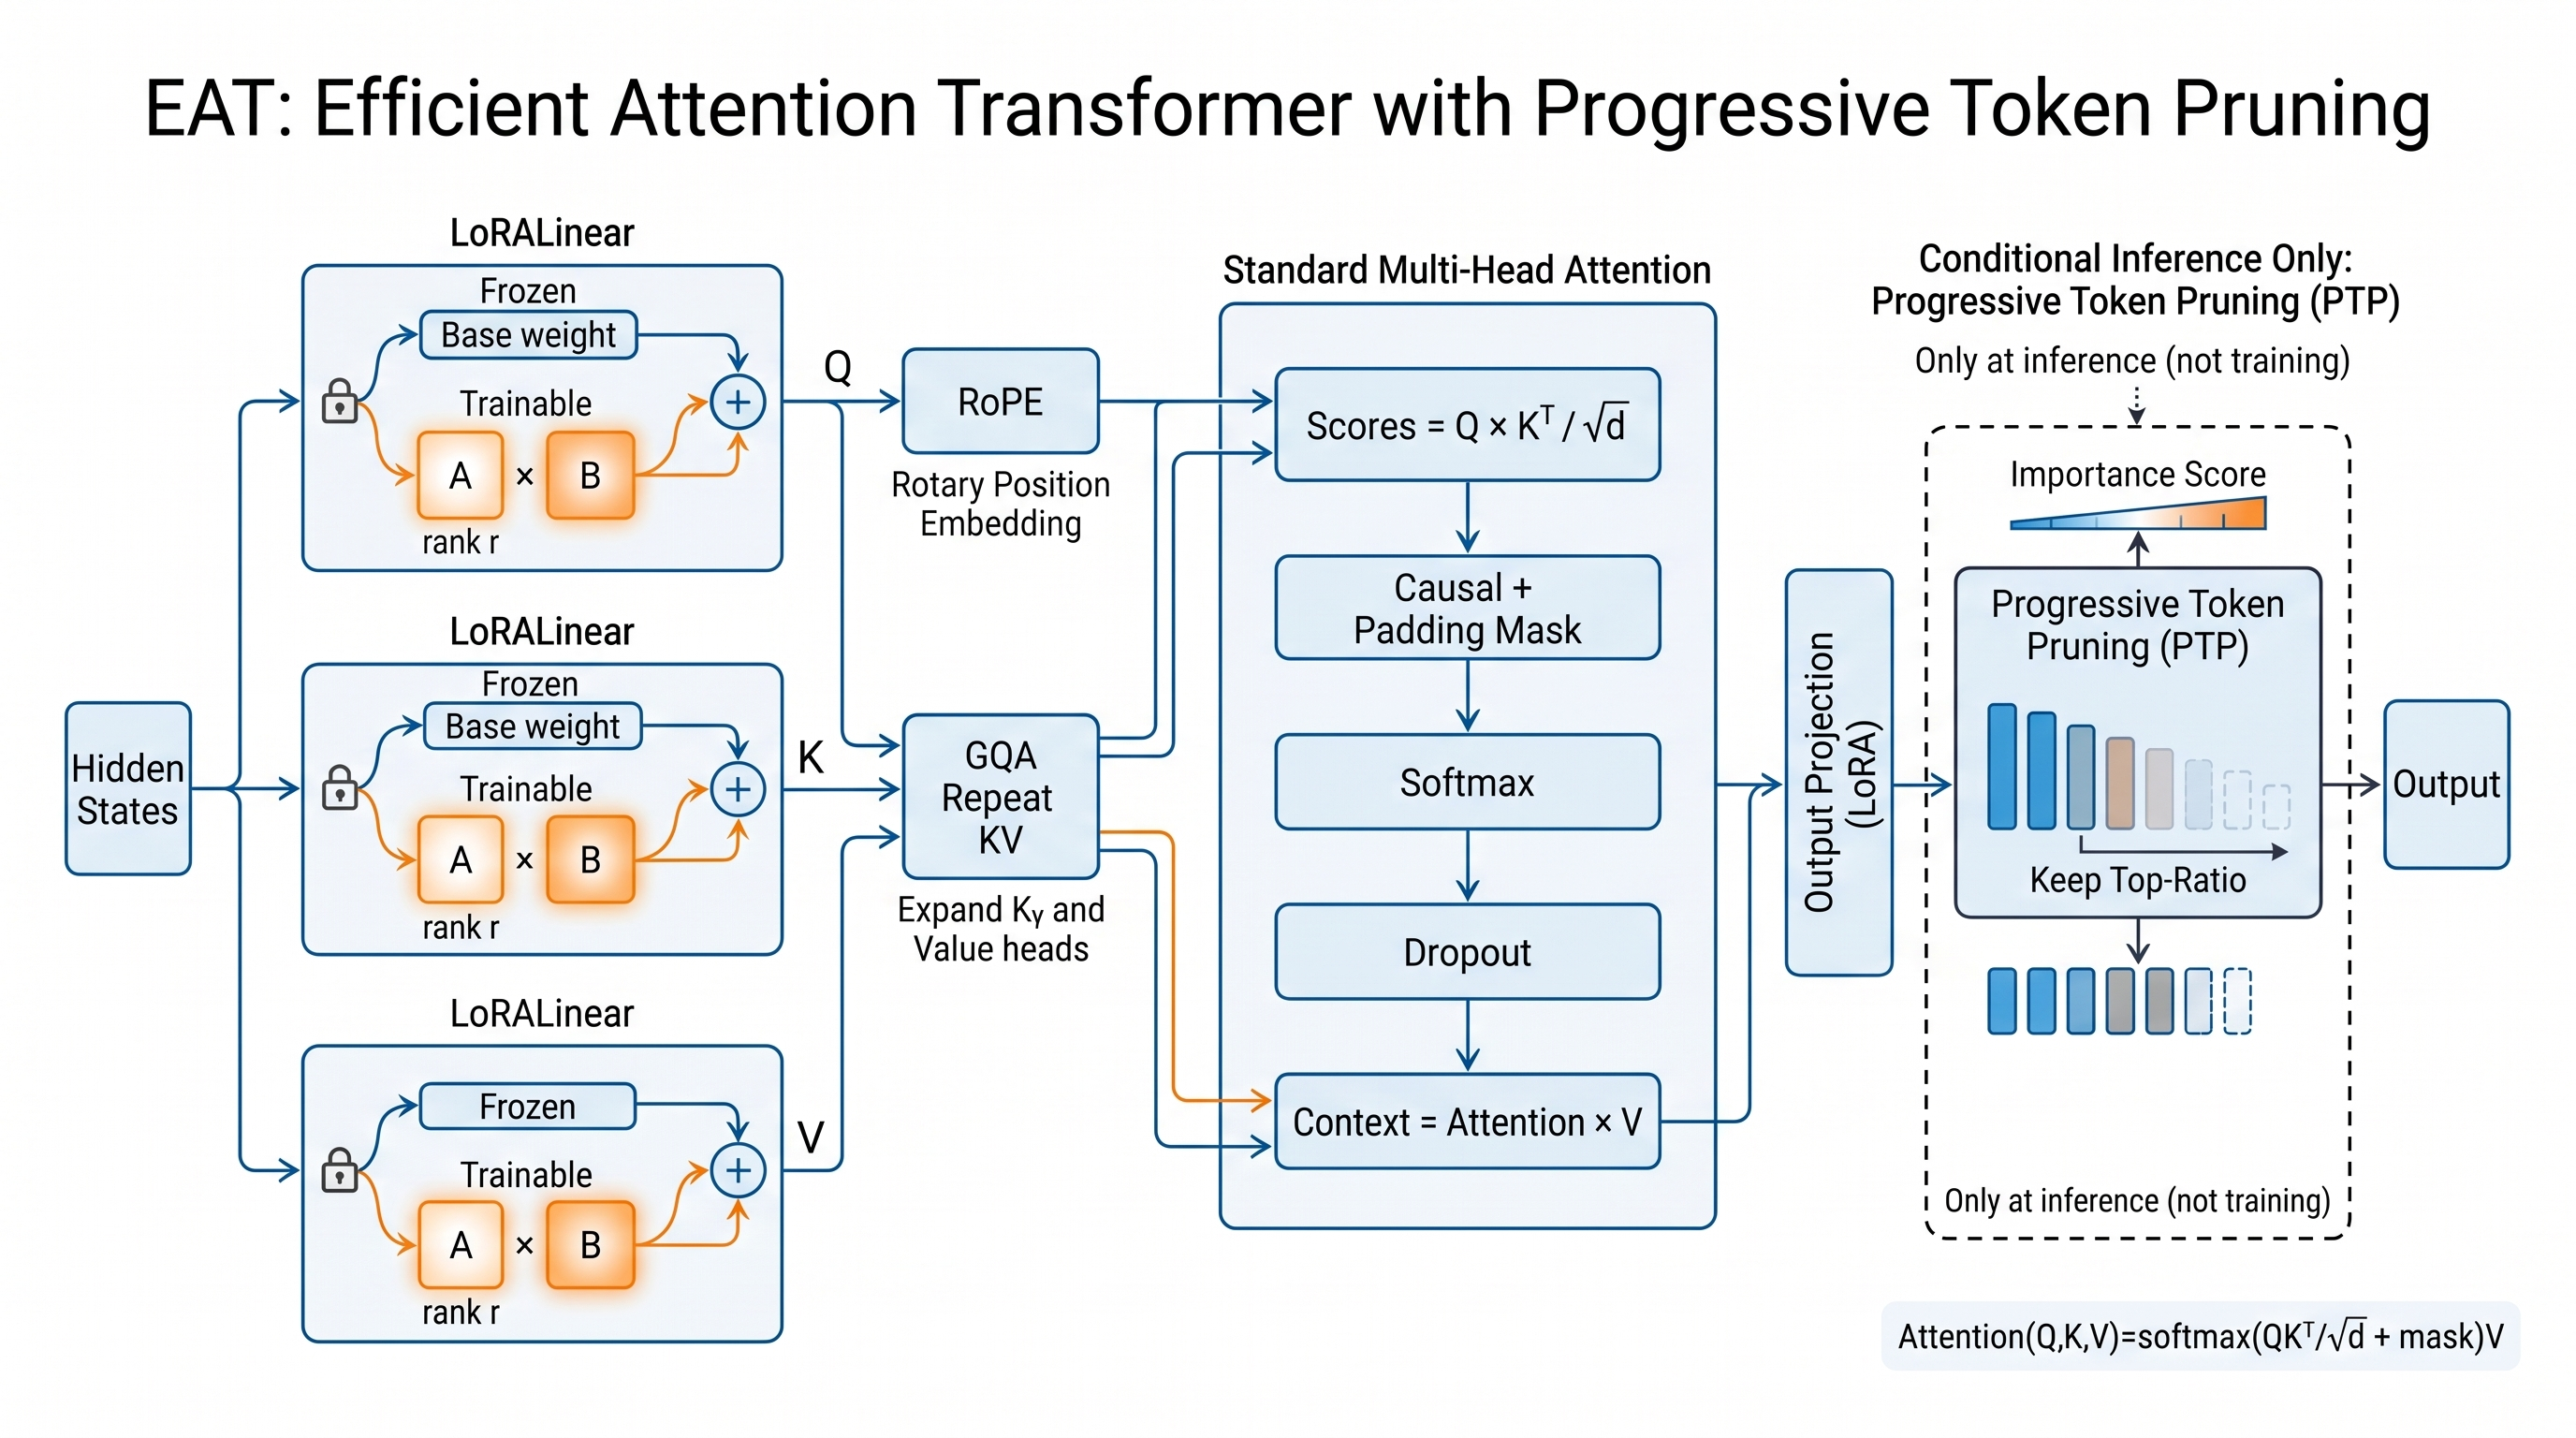
\includegraphics[width=\linewidth]{figures/architecture.jpeg}
\caption{High-level architectural diagram of eat.}
\label{fig:arch_eat}
\end{figure}

